\documentclass[10pt,twoside,twocolumn,openany]{dndbook}
\let\chaptername\relax

\usepackage[spanish]{babel}
\usepackage[utf8]{inputenc}
\usepackage[singlelinecheck=false]{caption}
\usepackage{listings}
\usepackage{shortvrb}
\usepackage{stfloats}
\usepackage{ifoddpage}
\usepackage{graphicx}
\usepackage{tikz}
\usepackage{fontawesome5} % Paquete para íconos
\usepackage{hyperref}

\hypersetup{
  colorlinks=true,
  linkcolor=black,  % Color de los enlaces internos (por ejemplo, dentro de la tabla de contenidos)
  urlcolor=magenta,   % Color de los enlaces a URLs
  %%citecolor=green,
  pdfauthor={Moisés Serrano Samudio},
  pdftitle={Luna de sangre},
  pdfsubject={one-shot},
  pdfkeywords={Dungeon and Dragons, DnD, 5e, secuestro, rescate}
}

\DndSetFonts[section-style = \linespread{.9} \color{titlered} \LARGE \scshape \RaggedRight]

\title{Luna de sangre\\
\large One shot para personajes de nivel inicial}
\author{linkmoises}
\date{\today}

\begin{document}

%% Portada
\newpage
\thispagestyle{empty}
\mbox{}
\begin{figure}
  \begin{tikzpicture}[remember picture,overlay]
    \begin{scope}
    \node [xshift=0cm,yshift=0cm] at (current page.center){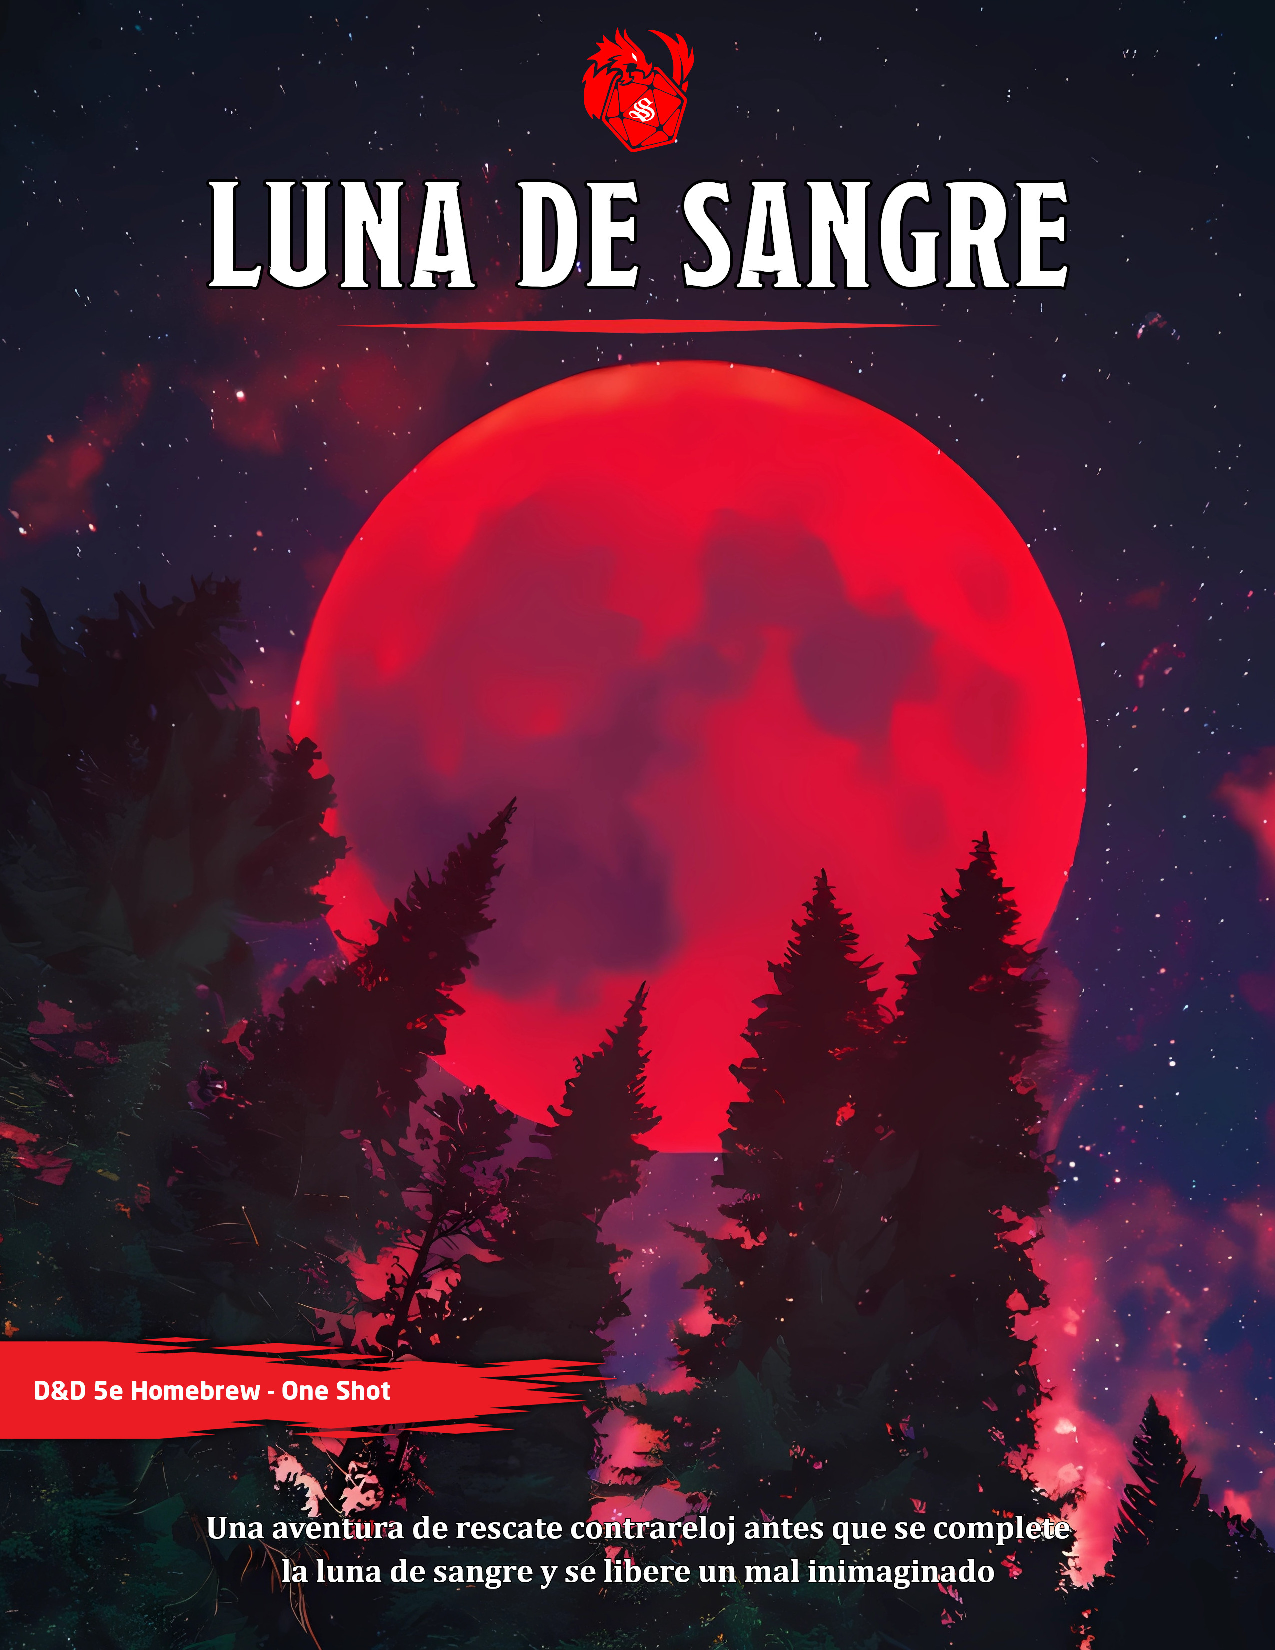
\includegraphics[width=\paperwidth]{covers/1-luna-de-sangre.jpg}};
    \end{scope}
  \end{tikzpicture}
\end{figure}
%% Finaliza portada

% hack para que texto de licencia se muestre en página siguiente
\newpage
\thispagestyle{empty}
\mbox{}

% Texto sobre la licencia CC-BY-SA
\newpage
\thispagestyle{empty} % Elimina el pie de página con numeración

\begin{center}
  \vspace*{\fill} % Ajustar espacio vertical antes del texto
  \begin{minipage}[b]{\textwidth}
      \justifying % Cambiar a justificado
      \noindent % Eliminar la sangría en la primera línea
      \faCreativeCommons \faCreativeCommonsBy \faCreativeCommonsNc \faCreativeCommonsSa \hspace{0.5em} 
      Contenido protegido por una \textbf{Licencia CC BY-NC-SA}
      \vspace{1em} % Espacio vertical entre título licencia y texto

      {\footnotesize
      \noindent
      El contenido escrito de este documento está protegido por la Licencia Creative Commons 
      Atribución-NoComercial-CompartirIgual 4.0 Internacional 
      \href{https://creativecommons.org/licenses/by-nc-sa/4.0/deed.es}{(CC BY-NC-SA)}. Esto 
      significa que puedes compartir, copiar, redistribuir, adaptar y crear a partir de este 
      contenido, siempre y cuando otorgues la debida atribución al autor original y compartas tus 
      derivados bajo una licencia similar que no permita el uso comercial. Las imágenes e 
      ilustraciones incluidas en este documento son creaciones de sus respectivos autores y están 
      protegidas por sus propias licencias. Consulta la sección créditos para obtener información 
      sobre las licencias individuales y conocer el trabajo de sus autores.
      }
    \end{minipage}
\end{center}

\frontmatter

\maketitle

\tableofcontents

\mainmatter

\part*{Luna de Sangre}

\chapter*{Sesión Cero}
\addcontentsline{toc}{chapter}{Sesión Cero}

\begin{tikzpicture}[remember picture, overlay]
  \node [xshift=0cm,yshift=-7cm] at (current page.north) {\includegraphics[width=\paperwidth]{media/zero.png}};
\end{tikzpicture}



\chapter*{Luna de Sangre}
\addcontentsline{toc}{chapter}{Luna de Sangre}

\DndDropCapLine{L}{as niñas de aldeas cerca de Phandalin} han estado desapareciendo en los 
últimos 3 días. Nadie sabe que está ocurriendo, solo se sabe que se acuestan y a la mañana 
siguiente ya no están. Los padres y madres preocupados ahora duermen en la misma habitación de
sus hijos o les amarran a la cama al momento de dormir para evitar que desaparezcan. La última 
niña en desaparecer fue la hija del gobernador hace solo unas horas. Han desaparecido un total de 
12 niñas en ese lapso de tiempo.

Desde entonces, el gobernador, Tormund Esses, ha colgado carteles por toda la aldea y en Phandalin 
ofreciendo recompensas por quién pueda dar información sobre el paradero de las niñas o las pueda 
encontrar.

\section{Presentación y gancho de aventura}

Los aventureros son aprendices de héroes que intentan ganar algo de fama y dinero. Varios aventureros 
se presentaron el último día para enfrentar el reto y encontrar a los niños. Por desgracia, ya sea 
por mala suerte o inexperiencia, hasta ahora no se sabe de ninguno de ellos.

Dependiendo de la conformación del grupo o del tiempo de disponible, la aventura puede ser abordada
permitiendo que el grupo explore las aldeas cercanas y que encuentren un rastro que se interne al 
bosque cercano. Queda a discreción del DM decidir cómo fueron capturados los jugadores y en qué 
momento. El grupo pudo ser emboscado o caer en alguna trampa y ser capturados. En todo caso,
los miembros del grupo llegan inconscientes a las celdas dónde los tienen prisioneros.

Los aventureros despertarán cerca de las diez de la noche, en celdas a la intemperie hechas por vigas de 
madera, algunos barrotes de hierro y sin ninguna de sus armas.


\section{Parte 1: Campamento Goblin}

A pesar de preferir ambientes oscuros y húmedos como cuevas, por alguna razón diferente a la usual 
un grupo de poco más de 20 goblins han establecido un campamento en las profundidades del bosque rodeado de 
árboles altos al lado de un río. Hay 5 tiendas improvisadas con una principal del doble de tamaño que 
las otras. La explanada del campamento ofrece un terreno bastante llano. Frente al campamento central, 
hay un pozo que ha sido excavado de manera circular rodeado por piedras con marcas rúnicas. 
Frente al foso, hay una mesa dispuesta como altar ceremonial.

Las celdas están ubicadas al sur del campamento y en su mayoría tienen 3 niñas por cada celda. Hay 
niñas asustadas en su mayoría, agotadas por la mala alimentación y deshidratadas algunas por qué 
están presentando vómitos y diarrea.

En la figura \ref{fig:camp1} se puede apreciar la disposición general del campamento goblin.

\begin{figure*}[hb!]
  \centering
  \includegraphics[width=\textwidth]{maps/goblin-camp.jpg}
  \caption{Campamento Goblin}
  \label{fig:camp1}
\end{figure*}

\begin{DndComment}{Prisioneros}
Los jugadores estarán repartidos de manera individual en cada celda. Cuando empiecen a preguntar qué 
ha pasado o donde están, podrán conseguir la siguiente información de un prisionero (perteneciente 
a una de las aldea) que llegó el día anterior al grupo, llamado Fred.

\begin{itemize}
    \item Todas las niñas desaparecidas están repartidos en las celdas y tienen 12 años.
    \item Los miembros del clan se escabullen en la noche y secuestran niños y niñas en sus casas en las aldeas cercanas.
    \item Un goblin grande encapuchado con la piel de color naranja dirige a los goblins. Su nombre es Grommash Tejesombras y dirige a los goblins con mano de hierro manteniéndolos aterrorizados.
    \item Grommash tiene una mascota, Sombrafauces, un perro del inframundo de tres cabezas, que alimenta con carne humana (y también de goblins). El chamán hobgoblin lo usa para intimidar a los goblins y a los prisioneros.
    \item Grommash se la pasa hablando de una luna de sangre.
\end{itemize}

\end{DndComment}

\DndArea{Tienda principal}
Se encuentra en el centro del campamento, es más grande y ornamentada que las otras, tiene una sola 
entrada y salida. Es custodiada siempre por dos goblins. En su interior, el piso es de piel de oso pardo 
y con una silla de madera tallada a manera de trono. Hay varios alijos de madera y un arcón de hierro 
dónde el clan guarda sus tesoros robados más importantes. Llama la atención una jaula de acero 
inmediatamente a la derecha luego de la entrada, dónde se encuentra Sombrafauces. Las paredes están 
cubiertas de pieles y trofeos de batalla. En el interior, los jugadores pueden encontrar un mapa 
detallado de la región, marcando lugares de interés y posibles aliados.

\DndArea{Pozo de sacrificios}
Esta área es un círculo excavado en el suelo, rodeado de piedras y adornado con runas oscuras. En esta 
área Grommash realiza sus rituales de sacrificio. Frente al pozo, los jugadores pueden encontrar 
una mesa ritual sobre la que hay un cuenco ritual, un cuchillo y un libro ritual.

\DndArea{Tiendas goblins}
Las tiendas improvisadas de los goblins son pequeñas y sucias, con literas apiladas en desorden. Hay 
varios catres de cuero, una mesa de madera improvisada donde colocan su equipo y varios barriles. 
Algunos goblins guardan pequeños tesoros personales en sus literas, como monedas de oro o joyas robadas.
En una de las literas, los jugadores pueden encontrar una carta escrita en un idioma desconocido que 
puede revelar información sobre los planes de Grommash. Cerca al río hay tres jaulas vacías con cadenas 
en su interior. Son usadas para amarrar a los huargos que montan los goblins que patrullan alrededor
del campamento.

\DndArea{Área de celdas}
Este lugar está rodeado por una empalizada de madera y alambre de púas. En el suelo de tierra, hay 
varias celdas rudimentarias, cada una con barrotes de hierro. 

\section{Eventos}
A medida que evoluciona la aventura, ocurrirán una serie de eventos que motivarán a los jugadores a 
tomar desiciones. Como evolucione la partida dependerá en gran parte de como los jugadores reaccionen 
luego de los dos eventos principales.

\begin{DndReadAloud}
  A medida que avanza la noche, los prisioneros caen en cuentra de la situación desesperada en la que 
  se encuentran. Grommash, el chamán hobgoblin se acerca a las improvisadas celdas diciendo en lengua 
  común, aún falta para la luna de sangre, pero tengo ganas de divertirme. Los mira a todos... 
  uno por uno, con una mirada que despierta un miedo interior que no habían sentido antes. Las niñas 
  se agitan en sus celdas. Luego a los pocos segundos se levanta su mano derecha con un índice acusador...
\end{DndReadAloud}

En este momento ha elegido a Fred. Fred, es un chico de 15 años. Fue testigo del rapto de una de las 
niñas, pero al seguir a los goblins que la llevaban, activó una de las trampas en el camino provocando 
así su propia captura.

\begin{DndReadAloud}
Los goblins sacan a Fred de su celda y lo llevan ante su jefe. Grommash le dice en lengua común, eres 
libre de irte muchacho. Tu vida no me interesa. Raudo y veloz, presa del miedo echa a correr hacia el 
oeste por el camino que lo habían traido. Cuando casi llegaba al límite del campamento con el bosque, 
Grommash dice "pero Sombrafauces no ha comido el día de hoy, a por él". Un aullido infernal retumbo 
en los oídos de los prisioneros y ven con horror como una sombra infernal como un perro de dos cabezas 
hace carrera detrás de Fred. Cuando ya se hubo internado en el bosque, unos segundos después escuchan 
gritos y luego silencio. Tras unos eternos minutos, emerge de las sombras, Sombrafauces. Lleno de sangre 
marcha hasta donde se encuentra su amo. Grommash dice en lengua común, aquellos que osen escapar 
sabrán a que atenerse.
\end{DndReadAloud}

La noche de la luna de sangre, Grommash empezará un ritual en el foso de sacrificios desde el inicio de la 
luna de sangre a las 11 de la noche. A partir de esta hora conducirá las niñas custodiadas por los 
goblins hacia el foso de los sacrificios. Grommash controlará telepáticamente, con ayuda de un 
amuleto que cuelga de su cuello con símbolos que dan cuenta que se trata de un objeto infernal, 
a una por una haciendo que se corte el cuello frente al altar improvisado y el foso de sacrificios. 
Una chica cada cinco minutos, mientras colecta la sangre que mana del cuello de sus víctimas en el 
cuenco ritual. Cuando la chica en cuestión comience a agonizar de pie, sus goblins la arrojarán al 
foso de sacrificios.

Que ocurra o no este último evento estará determinado por las acciones de los personajes jugadores.

\section{Conclusión}

Hay que destacar que si los jugadores intentan escapar a lo loco, confrontando directamente a los 
enemigos, lo más seguro es que acaben muertos. Los adversarios poseen una abundante ventaja numérica y 
podrían poner en un serio aprieto a los jugadores si optan por una estrategia directa.

Antes de iniciar el ritual, Grommash se encontrará en la tienda principal realizando algunos
rezos a sus deidades demoníacas preparandose para la luna de sangre.

Esta aventura está preparada para que los jugadores planeen su fuga y la del resto de las niñas prisioneras. 
Estos pueden intentar encargarse de algunos de los goblins, pero lo más seguro es que alguno muera por 
el camino si hay combates abiertos. Lo mejor será que los jugadores intenten acabar con los enemigos 
poco a poco, mediante subterfugios, intentando escapar de sus celdas y acabando con los goblins en 
pequeños grupos mientras descansan en sus tiendas.

Otras opciones serían escapar de las celdas sigilosamente (forzando la cerradura de la celda), envenenar 
a los goblins o asesinar por la noche a todos los goblins e intentarlo con Grommash. 

Los eventos de combate están pensados para que, de tener éxito, los jugadores se enfrenten poco a poco 
a todos los enemigos en cantidades asumibles, aunque podrían sufrir el desgaste, sobre todo de cara al 
último enfrentamiento.

Los jugadores superarán esta parte de la aventura si todos los miembros del campamento se han rendido 
o han sido muertos. Cómo recompensa obtendrán un item mágico del alijo de Grommash y recuperarán sus 
armas y armaduras básicas.


\section{Parte 2: Huida a la aldea}

Los jugadores deben escapar con las niñas del campamento y llevarlas sanas y salvas hasta la aldea. 
Antes de ello deberán sortear una serie de trampas que han dispuesto los goblins en el camino de salida. 
El campamento se halla unos 5 millas bosque adentro, en un terreno sumamente accidentado y que 
permanentemente esta cubierto de una niebla espesa. Con el escape ocurriendo durante la noche 
la temperatura fría del ambiente, condiciones de niebla densa y la luna de sangre ocurriendo dando 
un tono rojizo al ambiente, la visión estará limitada a unos 30 pies de distancia. La salida se 
encuentra al oeste del campamento.

\begin{DndReadAloud}
Mientras escapan hacia la aldea, cuando ya se han alejado unos 300 pies del campamento, escuchan 
un aullido gutural. Una brisa gélida, suave y ominosa se encuentra con los jugadores. La oscuridad
se cierra totalmente ante el grupo y el tono rojo que hay en el ambiente desaparece por un momento.
La tierra tiembla por un momento.
\end{DndReadAloud}

Unos goblins patrullan alrededor del campamento a unos 100 pies montados sobre huargos. Uno de ellos
se da cuenta de la huida y su huargo lanza un aullido alertando a otros.

Habrán 3 trampas dispuestas en el camino. La primera un foso cubierto por una enramada a 30 pies de e
la salida. Es posible que caigan si no superan una prueba de Sabiduría (percepción) superior a 15.

La segunda trampa es un sistema que lanza dardos qué están impregnados con un somnifero en sus puntas. 
Si alguno del grupo es alcanzado, ralentizara el avance como grupo, al obligar a cargar a los afectados 
y predisponiéndolos a ser alcanzados por los goblins montados en huargos y obligando al grupo a 
enfrentarlos.

Una tercera y última trampa estara esperándolos a 500 pies de la aldea. Se trata de otro foso cubierto
por una enramada y que es custodiado de manera oculta por 4 goblins arqueros del campamento desde los 
árboles esperando por cualquier incursión desde la aldea. 

Al llegar a la última trampa, son alcanzados por Grommash quien va montado sobre Sombrafauces.
Sombrafauces ha crecido en tamaño dos veces de la última vez que lo vieron. Grommash se ha desplazado
utilizando Teletransportación sombría. Grommash tiene un aura oscura y una mirada que recuerda las llamas 
infernales. Al realizar el ritual de luna de sangre ganó una acción legendaria.

\section{Conclusión}

Los jugadores superarán esta parte de la aventura si logran llegar a la aldea con las niñas. Si logran 
llegar con las 12 niñas recibirán una recompensa de 100 piezas de oro cada uno. Si muere alguna de las 
niñas recibirán una recompensa de 50 piezas de oro para todo el grupo.

\section{Créditos}

Las ilustraciones en este one shot, son creaciones de sus respectivos autores. Los mapas han sido 
creados con la herramienta \href{https://inkarnate.com/}{Inkarnate}. Estos son los enlaces a las 
ilustraciones originales:

\begin{itemize}
  \item Grommash Tejesombras por \href{https://legendofthecryptids.fandom.com/wiki/Greedy_Goblin_King}{Hua Lu: Greedy Goblin King para el juego de cartas Legends of Cryptids}.
  \item Sombrafauces \href{https://www.deviantart.com/lucy-lisett/art/Death-Dog-901248620}{Lucy-Lisett Hell Dog en Deviantart creado el para TTRPG Blood \& Doom}.
  \item Goblin Camp por \href{https://inkarnate.com/m/zkNwn5--goblin-camp/}{DMMarty en Inkarnate} modificado por linkmoises para este one shot.
\end{itemize}

%%
%%
%%
\part*{Apéndice de monstruos}
%%
%%
%%

\chapter*{Grommash}
\addcontentsline{toc}{chapter}{Grommash Tejesombras}


\begin{tikzpicture}[remember picture, overlay]
    \node[anchor=north west] at ([xshift=-0.5cm,yshift=0.5cm]current page.north west){\includegraphics[scale=3.6]{media/chaman-hobgoblin.png}};
\end{tikzpicture}


% Monster stat block
\begin{DndMonster}[float*=b,width=\textwidth + 8pt]{Grommash Tejesombras}
    \begin{multicols}{2}
        \DndMonsterType{Chamán hobgoblin, caótico malvado}

    % If you want to use commas in the key values, enclose the values in braces.
    \DndMonsterBasics[
	armor-class = {12 con \emph{armadura de cuero}},
        hit-points  = {\DndDice{3d8 + 3}},
        speed       = {30 ft},
      ]

    \DndMonsterAbilityScores[
        str = 13,
        dex = 14,
        con = 13,
        int = 10,
        wis = 10,
        cha = 8,
      ]

    \DndMonsterDetails[
        %saving-throws = {Str +0, Dex +0, Con +0, Int +0, Wis +0, Cha +0},
        %skills = {Acrobatics +0, Animal Handling +0, Arcana +0, Athletics +0, Deception +0, History +0, Insight +0, Intimidation +0, Investigation +0, Medicine +0, Nature +0, Perception +0, Performance +0, Persuasion +0, Religion +0, Sleight of Hand +0, Stealth +0, Survival +0},
        %damage-vulnerabilities = {cold},
        %damage-resistances = {bludgeoning, piercing, and slashing from nonmagical attacks},
        %damage-immunities = {poison},
        %condition-immunities = {poisoned},
        senses = {visión en la oscuridad 120 pies, percepción pasiva 10},
        languages = {común, goblin, infernal},
        challenge = 3,
      ]
    % Traits
    \DndMonsterAction{Llamas infernales}
    Grommash puede lanzar llamas infernales en un área, causando daño de fuego a los enemigos cercanos.
    % \begin{DndMonsterSpells}
    %   \DndInnateSpellLevel{misty step}
    %   \DndInnateSpellLevel[3]{fog cloud, rope trick}
    %   \DndInnateSpellLevel[1]{identify}
    % \end{DndMonsterSpells}

    \DndMonsterAction{Teletransportación sombría}
    Puede usar una teletransportación sombría para moverse rápidamente a través de la oscuridad y aparecer en un 
    lugar diferente.

    \DndMonsterAction{Maleficio maldito}
    Maleficio Maldito: Puede lanzar un maleficio maldito sobre un objetivo, haciéndolo más vulnerable a los ataques.

    \DndMonsterSection{Acciones}
    \DndMonsterAction{Ataque con bastón mágico}
    Grommash puede usar su bastón mágico para lanzar rayos de energía a larga distancia o como arma de 
    combate cuerpo a cuerpo.

    \DndMonsterAction{Grito de guerra}
    Grommash emite un aterrador grito de guerra que inspira a sus seguidores goblins, dándoles un impulso 
    temporal en el combate.

    % %Default values are shown commented out
    % \DndMonsterAttack[
    %   name=Dagger,
    %   %distance=both, % valid options are in the set {both,melee,ranged},
    %   %type=weapon, %valid options are in the set {weapon,spell}
    %   mod=+3,
    %   %reach=5,
    %   %range=20/60,
    %   %targets=one target,
    %   dmg=\DndDice{1d4+1},
    %   dmg-type=piercing,
    %   %plus-dmg=,
    %   %plus-dmg-type=,
    %   %or-dmg=,
    %   %or-dmg-when=,
    %   %extra=,
    % ]

    % %\DndMonsterMelee calls \DndMonsterAttack with the melee option
    % \DndMonsterMelee[
    %   name=Flame Tongue Longsword,
    %   mod=+3,
    %   %reach=5,
    %   %targets=one target,
    %   dmg=\DndDice{1d8+1},
    %   dmg-type=slashing,
    %   plus-dmg=\DndDice{2d6},
    %   plus-dmg-type=fire,
    %   or-dmg=\DndDice{1d10+1},
    %   or-dmg-when=if used with two hands,
    %   %extra=,
    % ]

    % %\DndMonsterRanged calls \DndMonsterAttack with the ranged option
    % \DndMonsterRanged[
    %   name=Assassin's Light Crossbow,
    %   mod=+1,
    %   range=80/320,
    %   dmg=\DndDice{1d8},
    %   dmg-type=piercing,
    %   %plus-dmg=,
    %   %plus-dmg-type=,
    %   %or-dmg=,
    %   %or-dmg-when=,
    %   extra={, and the target must make a DC 15 Constitution saving throw, taking 24 (7d6) poison damage on a failed save, or half as much damage on a successful one}
    % ]

    \DndMonsterSection{Reacciones}
    \DndMonsterAction{Escudo arcano}
    Grommash puede reaccionar ante un ataque inminente creando un escudo arcano que reduce el daño recibido.

    \DndMonsterAction{Maldición vengativa}
    Si un enemigo le causa un daño significativo, Grommash puede lanzar una maldición vengativa sobre ese enemigo, 
    haciéndolo más vulnerable a futuros ataques.

    % Legendary Actions
    \DndMonsterSection{Acciones legendarias}
    Si Grommash logra completar el ritual de la luna de sangre, su poder se incrementa. Sus puntos de golpe y su CA se 
    multiplican por 10. Si logra sacrificar alguna de las niñas sus puntos de golpe y CA se multiplican por 2. Si sacrifica uno
    de los goblins en el foso de los sacrificios recupera la mitad de sus puntos de golpe y CA. En todo caso, realizar el 
    ritual de forma completa o parcial le permite lanzar una poderosa acción legendaria llamada ``Apoteosis de Sangre''. 
    Cuando activa esta acción, el cielo se oscurece totalmente y la tierra tiembla mientras canaliza la energía de la luna 
    de sangre.

    \begin{DndMonsterLegendaryActions}
      \DndMonsterLegendaryAction{Ataque devastador}{Grommash puede realizar un ataque devastador de área que inflige daño a todos los objetivos en un radio de 30 pies alrededor de él. Este ataque es una explosión de energía mágica en forma de una llamarada de fuego infernal.}
      \DndMonsterLegendaryAction{Parálisis temporal}{Todos los objetivos afectados por esta acción deben hacer una tirada de salvación contra una maldición que produce una parálisis temporal debido a la abrumadora presencia de Grommash.}
    \end{DndMonsterLegendaryActions}
  \end{multicols}
\end{DndMonster}


\chapter*{Sombrafauces}
\addcontentsline{toc}{chapter}{Sombrafauces}


\begin{tikzpicture}[remember picture, overlay]
    \node[anchor=north west] at ([xshift=-0.5cm,yshift=0.5cm]current page.north west){\includegraphics[scale=3.6]{media/hell-dog.png}};
\end{tikzpicture}


% Monster stat block
\begin{DndMonster}[float*=b,width=\textwidth + 8pt]{Sombrafauces - perro del inframundo}
    \begin{multicols}{2}
        \DndMonsterType{Monstruosidad mediana, caótico malvado}

    % If you want to use commas in the key values, enclose the values in braces.
    \DndMonsterBasics[
        armor-class = {12},
        hit-points  = {\DndDice{6d8 + 12}},
        speed       = {40 ft},
      ]

    \DndMonsterAbilityScores[
        str = 15,
        dex = 14,
        con = 14,
        int = 3,
        wis = 13,
        cha = 6,
      ]

    \DndMonsterDetails[
        %saving-throws = {Str +0, Dex +0, Con +0, Int +0, Wis +0, Cha +0},
        %skills = {Acrobatics +0, Animal Handling +0, Arcana +0, Athletics +0, Deception +0, History +0, Insight +0, Intimidation +0, Investigation +0, Medicine +0, Nature +0, Perception +0, Performance +0, Persuasion +0, Religion +0, Sleight of Hand +0, Stealth +0, Survival +0},
        %damage-vulnerabilities = {cold},
        %damage-resistances = {bludgeoning, piercing, and slashing from nonmagical attacks},
        %damage-immunities = {poison},
        %condition-immunities = {poisoned},
        senses = {visión en la oscuridad 120 pies, percepción pasiva 15},
        languages = {entiende infernal, pero no lo habla},
        challenge = 3,
      ]
    % Traits
    \DndMonsterAction{Teletransportación sombría}
    Puede ser teletransportado junto a Grommash Tejesombras a través de la oscuridad.

    \DndMonsterAction{Tres cabezas}
    El perro tiene ventaja en las pruebas de Sabiduría (Percepción) y en las tiradas de salvación para evitar ser
    asustado, aturdido, cegado, ensordecido, hechizado o dejado inconsciente.

    \DndMonsterSection{Acciones}
    \DndMonsterAction{Ataque múltiple}
    El perro realiza tres ataques de mordisco.

    %Default values are shown commented out
    \DndMonsterAttack[
      name=Mordisco,
      distance=melee, % valid options are in the set {both,melee,ranged},
      %type=weapon, %valid options are in the set {weapon,spell}
      mod=+4,
      reach=5,
      %range=20/60,
      targets=un objetivo,
      dmg=\DndDice{1d6+2},
      dmg-type=perforante,
      %plus-dmg=,
      %plus-dmg-type=,
      %or-dmg=,
      %or-dmg-when=,
      extra={. Si el objetivo es una criatura, debe superar una tirada de salvación de Constitución CD 12 contra enfermedad para no quedar envenenado hasta que se cure la enfermedad. Cada 24 horas, la criatura debe repetir la tirada de salvación y, si falla, su máximo de puntos de golpe se reduce en 5 (1d10). Esta reducción dura hasta que se cure la enfermedad. La criatura muere si la enfermedad reduce su máximo de puntos de golpe a 0},
    ]
  

  \end{multicols}
\end{DndMonster}

% hack para que contraportada se muestre en página siguiente
\newpage
\mbox{}

\newpage
\thispagestyle{empty}
\mbox{}

\begin{figure}
  \begin{tikzpicture}[remember picture,overlay]
    \begin{scope}
    \node [xshift=0cm,yshift=0cm] at (current page.center){\includegraphics[width=\paperwidth]{covers/contraportada.jpg}};
    \end{scope}
  \end{tikzpicture}
\end{figure}

\end{document}